\documentclass[11pt,a4paper,oneside,BCOR=0cm,DIV=13]{scrartcl}

\title{L'angélus}
\author{}
\usepackage{fontspec}
\usepackage{polyglossia}
\usepackage{hyperref}

\setdefaultlanguage{latine}

\setmainfont[Mapping=tex-text,Style=Swash,Numbers={OldStyle,Proportional},Ligatures={Rare,Historic}]{EB Garamond}
%\setmainfont[Ligatures=TeX]{Linux Libertine O}
\setsansfont[Mapping=tex-text,Style=Swash,Numbers={OldStyle,Proportional},Ligatures={Rare,Historic}]{EB Garamond}


\usepackage[autocompile]{gregoriotex}
\usepackage{fancyhdr}
 
\pagestyle{empty}
\KOMAoptions{DIV=last}
\begin{document}
\begin{center}
\Huge \textsc{L'angélus}
\vspace{0.4cm}

\normalsize \small \emph{CC† -- CentraleSupélec - campus de Metz.} \\ \small Version du 1\textup{er} décembre 2015. \\ \small Sous licence CC BY (Luc Absil). \\\href{http://cccroix.github.io}{\texttt{cccroix.github.io}}
\end{center}

\vspace{1cm}

{\flushright\emph{Par Dom Charpentier.} \small-- transcription : Luc Absil\\}

\includescore{angelus1}
\vspace{1cm}

\begin{center}
{\small
\begin{tabular}{p{5cm} p{5cm}}
\textbf{Oremus}. Gratiam tuam quæsumus, Domine, mentibus nostris infunde; ut qui, angelo nuntiante, Christi Filii tui Incarnationem cognovimus, per passionem eius et crucem, ad resurrectionis gloriam perducamur. Per eumdem Christum Dominum nostrum. 

Amen.

Gloria Patri...
&
\textbf{Prions}. Daignez, Seigneur, répandre votre grâce dans nos âmes, afin qu'ayant connu par la voix de l'Ange l'Incarnation de Votre Fils Jésus Christ, nous puissions parvenir par sa Passion et par sa Croix, à la gloire de sa Résurrection, par le même Jésus Christ Votre Fils, notre Seigneur. 

Amen

Gloire au Père...
\end{tabular}
}
\end{center}

\newpage
\section*{Ave Maria}

\vspace{1cm}

{\flushright Liber Usualis (\emph{Solesmes}). \small-- transcription : Andrew Hinkley\\}

\includescore{ave_maria_solesmes}

\begin{center}
\vspace{4cm}
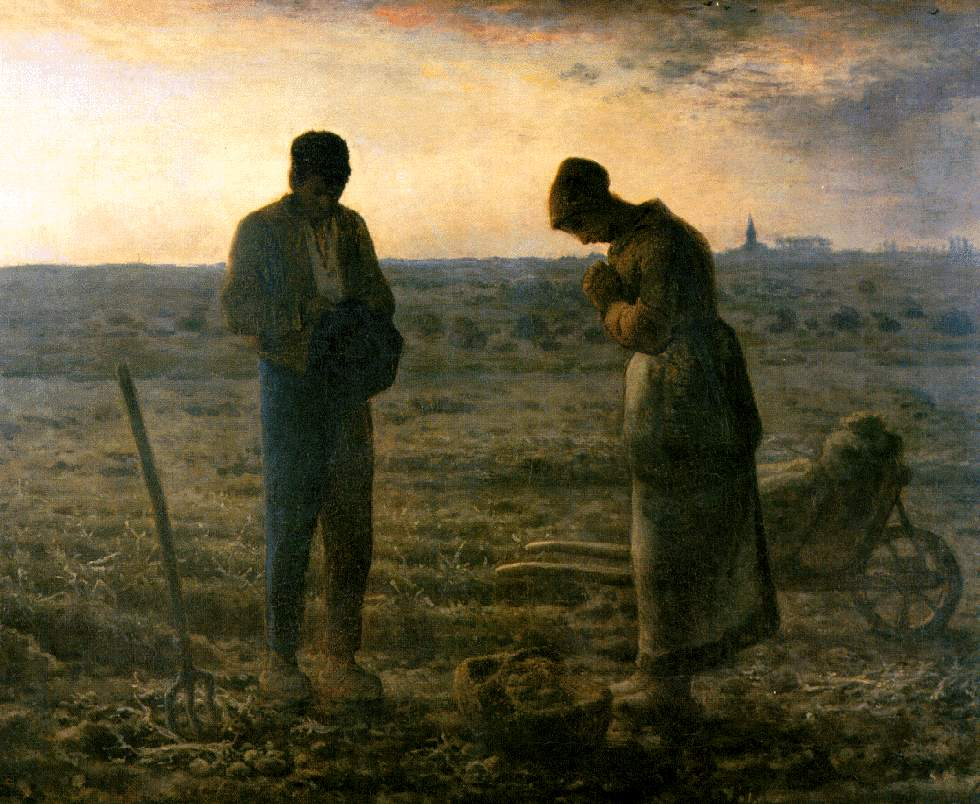
\includegraphics[width=9cm]{Millet.jpg}
~\\
\emph{L'Angelus}, Millet, 1859\\ (\emph{{\small image wikicommons}})
\end{center}
\end{document} 
